\documentclass[format=acmsmall]{acmart}
\begin{document}
\title{GPU-friendly Stroke Expansion}
\author{Raph Levien}
\author{Arman Uguray}
\affiliation{
    \institution{Google}
    \city{San Francisco}
    \state{CA}
    \country{USA}
}

\begin{abstract}
    Vector graphics includes both filled and stroked paths as the main primitives. While there have been many proposed techniques for rendering filled paths on GPU, stroked paths have proved more elusive. This paper presents a technique for performing stroke expansion, namely the generation of an outline representing the stroke of the given input path, an operation which is considered global, but which we nonetheless implement using a fully parallel algorithm. We introduce several novel techniques, including an encoding of stroked primitives suitable for parallel processing and an Euler spiral based method for computing both flattened parallel curves and approximations to arc segments. Our method produces a near-optimal number of line segments for the filled outline of a stroked cubic Bézier and can be fully evaluated on a GPU with minimal preprocessing.
\end{abstract}

\maketitle
\thispagestyle{empty}
\pagestyle{plain}

\section{Introduction}

Rendering of vector graphics documents requires handling both filled and stroked primitives. There is substantial literature on GPU rendering of filled paths, but many fewer published techniques for strokes. It is a more challenging problem, especially for parallel computation, because path segments cannot be processed independently of each other; the \emph{joins} between adjacent path segments depend on context. In addition, the path topology affects the rendered result, in particular whether subpaths are open or closed. In the former case, the endpoints are rendered with \emph{caps}. Joins and caps can have multiple styles, including different styles within the same document.

TODO: brief description of stroke to fill conversion.

The \cite{Nehab2020} paper gives a comprehensive survey of techniques for stroke expansion, and an algorithm which, for a number of reasons, is only suitable for implementation on CPU (though adapting it to GPU is listed as promising future work). It classifies techniques into \emph{local,} where each path segment generates closed geometry (which may be triangles or other primitives), and \emph{global,} where the overall result is a closed outline of the stroked path, but the partial result from each segment is in general open. Our technique is considered global in this scheme, yet allows independent processing of each path segment.

A number of factors contribute to an algorithm being ``GPU-friendly.'' In addition to simply being able to process the input segments in parallel, such an algorithm also avoids divergent control flow (avoiding the need for explicit subdivision at special events such as inflection points and cusps) and uses robust numerical techniques not subject to particular problems when evaluated using 32-bit floating point numbers.

We propose that the correctness of stroke outlines be divided into \emph{weak correctness} and \emph{strong correctness.} We define strong correctness as the computation of the outline of a line swept along the segment, maintaining normal orientation, combined with stroke caps and joins. Weak correctness, by contrast, only requires the parallel curves of stroke segments, combined with caps and the outer contours of joins. The two notions are equivalent for sufficiently well-behaved input, in particular when the curvature measured at endpoints of path segments does not exceed the reciprocal of the half linewidth. As described in detail in \cite{Nehab2020}, very few existing implementations actually implement the strong version, so document authors have become accustomed to not depending on behavior at endpoints. Standards for graphics formats also provide an ``out,'' enabling the weaker behavior. [TODO: find language in SVG standard]. While our current implementation emphasizes weak correctness, we believe it can be extended to the stronger sense, by implementing evolutes and inner join contours.

TODO: discussion of prior art.

\begin{itemize}
    \item Nehab 2020
    \item Kilgard 2020: Polar stroking (discussion of error metric can move here)
    \item Yzerman 2020: combined offset + flatten using quadratics
    \item Blog post of Dragoș?
    \item Curve-to-curve offsetting? Tiller and Hanson (which is good for quadratics, terrible for cubics), Shape control (pretty good but has robustness issues). Hain (misses error tolerance in cusp case, as described in Yzerman). The "Comparing Offset Curve Approximation Methods" paper is flawed.
\end{itemize}

\section{Input encoding}

One contribution of this paper is a highly efficient encoding for paths to be rendered. Goals include conciseness, low cost to encode on the CPU side, and fully parallel processing by the GPU. There are two major aspects to the encoding: a variable size encoding of paths, suitable for both filling and stroking, and an extension to stroking. The input is separated into a \emph{tag stream}, with one byte per path element, and another stream for the coordinate data. The index into coordinate data is computed by a prefix sum from a size value derived from the tag byte.

\subsection{Path encoding}

The tag byte is a number of bit fields, packed into a byte.

TODO: make this into a diagram.

\begin{itemize}
    \item 0-1: coordinate count
    \item 2: subpath end bit
    \item 3: 16/32 bit coordinates
    \item 4: path end bit
    \item 5: transform bit
    \item 6: line style bit
\end{itemize}

For most path segments, the coordinate count indicates the type of path segment: 1 for lines, 2 for quadratic Beziers, and 3 for cubic Beziers. The subpath bit is set on the last segment of a subpath, and the path bit is additionally set on the last bit of a path. The latter is not directly interpreted by the path flattening code, but is forwarded to later rendering stages, for example, the path id can be used to select a color or other paint style.

The size is readily inferred from the tag byte: the number of coordinate pairs is the coordinate count plus one if the subpath end bit is set. The nuber of bytes per coordinate pair is 4 for 16 bit coordinates or 8 for 32 bit coordinates.

It is relatively straightforward to convert the standard moveto/lineto/curveto path representation into this encoding. Subpath boundaries are moved from the beginning of a subpath (moveto) to the end. A separate segment must be generated for closepath if the ending point does not coincide with the start point.

The handling of the subpath bit allows for overlap in coordinates, so that, except at subpath boundaries, the first coordinate pair of each path segment overlaps with the last coordinate pair of the previous one. Subpath handling is all computed in the prefix sum; no special handling is needed on the GPU side.

\section{Flattening and arc approximation of curves}

% Note: this is being written as a fairly stand-alone section. No doubt some reorganization should happen

The core problem in stroke expansion is approximating the desired curve by segments of some other curve, usually a simpler one. These segments must be within an error tolerance of the source curve, and ideally there are not many more of them than optimal. We consider a number of source to target pairs, most importantly cubic Béziers to Euler spirals, and Euler spiral parallel curves to either lines or arcs.

There are generally three approaches to such curve approximation. The most straightforward but also least efficient is ``cut then measure,'' usually combined with adaptive subdivision. In this technique, a candidate approximate curve is produced, then the error is measured against the source curve, usually by sampling a number of points along both curves and determining a maximum error (or perhaps some other error norm). If the error is within tolerance, the approximation is accepted. Otherwise, the curve is subdivided (usually at t = 0.5) and each half is recursively approximated. A substantial fraction of all curve approximation methods in the literature are of this form, including \cite{Nehab2020}. The main disadvantage is the cost of computing the error metric. Another risk is underestimating the error due to inadequate sampling; this is a particular problem when the source curve contains a cusp.

% Note: would be cool to run profiler on Nehab code to determine fraction of time computing error metric.

The next approach is similar, but uses an \emph{error metric} to estimate the error. Ideally such a metric is a closed-form computation rather than requiring iteration. A good error metric is conservative, yet tight, in that it never underestimates the error (which would allow results exceeding the error bound to slip through), and does not significantly overestimate the error, which would result in more subdivision than optimal.

By far the most efficient approach is an \emph{invertible} error metric. In this approach, the error metric has an analytic inverse, or at least a good numerical approximation. Because the metric is invertible, it can predict the number of subdivisions needed, as well as the parameter value for each subdivision. If the error metric is accurate, then approximation is near-optimal. One example of an invertible error metric is angle step, used in polar stroking\cite{Kilgard2020}; the number of subdivisions is the total angle subsumed by the curve divided by the angle step size, and the parameter value for each subdivision is the result of solving for a tangent direction. Another widely used invertible error metric is Wang's formula (\cite{Goldman2003}, Section 5.6.3), which gives a bound on the flattening error based on the second derivative of the curve. This metric is conservative but works well in practice; among other applications, it is used in Skia for path flattening. One limitation of Wang's method is that it only applies to the flattening of filled outlines, not parallel curves as is required for strokes.

% Note: an alternate cite for the central result of Wang's formula is Sederberg's lecture notes. It doesn't use the name "Wang's formula." In one way, it is a cleaner result, as it doesn't have the rounding up to a power of 2. But it is also less of an archival cite.
% https://scholarsarchive.byu.edu/cgi/viewcontent.cgi?article=1000&context=facpub#section.10.6

\subsection{Error metrics for flattening}

The distance between a circular arc segment of length $s$, with angle between arc and chord of $\theta$ (see Figure~\ref{fig:arc_chord}), is exactly $(1-\cos \theta)s/(2\theta)$. The curvature is $\kappa = \frac{2\theta}{s}$ (equivalently, $\theta = \frac{\kappa s}{2s}$), and this remains constant even as the arc is subdivided. Rewriting, $d = (1-\cos\frac{\kappa}{2s})\frac{s}{\kappa}$. From this, we can derive a precise, invertible error metric. Subdividing the arc in to $n$ segments, the distance error for each segment is $\frac{1}{\kappa}(1-\cos \frac{s\kappa}{2n})$. Solving for n, we get:

\begin{figure}
    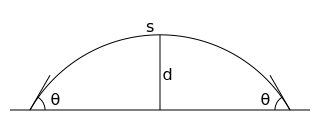
\includegraphics[scale=0.5]{arc_chord}
    \caption{A circular arc segment with notations for angles ($\theta$), arc length ($s$), and distance to chord ($d$)}
    \Description{A circular arc above its chord, with labels at the endpoints for angle from chord ($\theta$), the length of the arc ($s$) and the maximum distance from the arc to its chord ($d$).}
    \label{fig:arc_chord}
\end{figure}

% TODO: I might supplement this figure with one subdivided with n=3

\[
n = \frac{s\kappa}{2\cos^{-1}\left( 1- d\kappa \right)}
\]

To flatten a finite arc, round up $n$ to the nearest integer. This will cause the error to decrease, so will still be within the error bounds.

Note that the number of subdivisions is proportional to the arc length. Another way of stating this relationship is that the \emph{subdivision density}, the number of subdivisions per unit of arc length, is constant.

The error metric for flattening an arc is exact. It always yields the minimum number of subdivisions needed to flatten the curve, and the flattening error is the least possible with given that number of subdivisions. For general curves, an exact error bound is not feasible, and we resort to an approximation. Again the circular arc provides a good example. Applying the small angle approximation $\cos \theta \approx 1 - \theta^2/2$, the approximate distance error is $d = \frac{\kappa s^2}{8n^2}$, and solving for $n$ we get $n = s\sqrt{\frac{\kappa}{8d}}$. Note that this estimate is \emph{conservative,} in that it will always request more subdivision and thus produce a lower error than the exact metric.

We are of course concerned with the flattening of more general curves (ultimately the parallel curve of a cubic Bézier), not simply circular arcs. It is tempting to sample the curvature and plug it into the formula above, but this can both dramatically undershoot the error (predicting that no subdivision is needed at an inflection point) and overshoot it (requiring infinite subdivision at a cusp; and cusps). Apparently, some kind of average curvature is needed.

We propose the following error metric to estimate the maximum distance between an arbitrary curve of length $\hat{s}$ and its chord. 

\[
    d \approx \frac{1}{8}\left(\int_0^{\hat{s}} \sqrt{|\kappa(s)|}ds \right)^2
\]

% Should s-hat be the integration variable instead? Is there a better choice of symbol?

This formula is the same as the approximate error metric for circular arcs, except that instead of a constant curvature value, a norm-like average with an exponent of 1/2 is used (it is not considered a true norm because the triangle inequality does not hold). We chose this particular formulation because it tends to produce invertible error metrics, and because it works well in practice.

This formula also has a meaningful interpretation: the quantity under the integral sign is the subdivision density, and represents the number of subdivisions per unit length of an optimal flattening as the error tolerance approaches zero. In particular, the number of subdivisions is:

\[
    n = \left(\int_0^{\hat{s}} \sqrt{|\kappa(s)|}ds \right)\sqrt{\frac{1}{8d}}
\]

In addition, if the function represented by the integral is invertible, then the corresponding error metric is invertible. Evaluate the function to determine the number of subdivision points, then evenly divide the result, using the inverse of the function to map these values back into parameter values for the source curve being approximated.

\subsection{Error metrics for flattening Euler spirals}

We choose Euler spiral segments for our intermediate curve representation precisely because their simple formulation in terms of curvature (Cesàro equation) results in similarly simple subdivision density integrals.

An Euler spiral segment is defined by $\kappa(s) = as+b$, or alternatively $\kappa(s) = a(s-s_0)$, where $s_0 = -b/a$ is the location of the inflection point. Applying the above error metric, the subdivision density is simply $\sqrt{|a(s-s_0)|}$. The integral is $\frac{2}{3}\sqrt{a}(s-s_0)^{1.5}$, which is readily invertible.

An immediate consequence is that flattening an Euler spiral by choosing subdivision points $s_i = a\cdot i^\frac{2}{3}$ produces a near-optimal flattening, as can visually be seen in Figure\ref{fig:es_flatten}.

\begin{figure}
    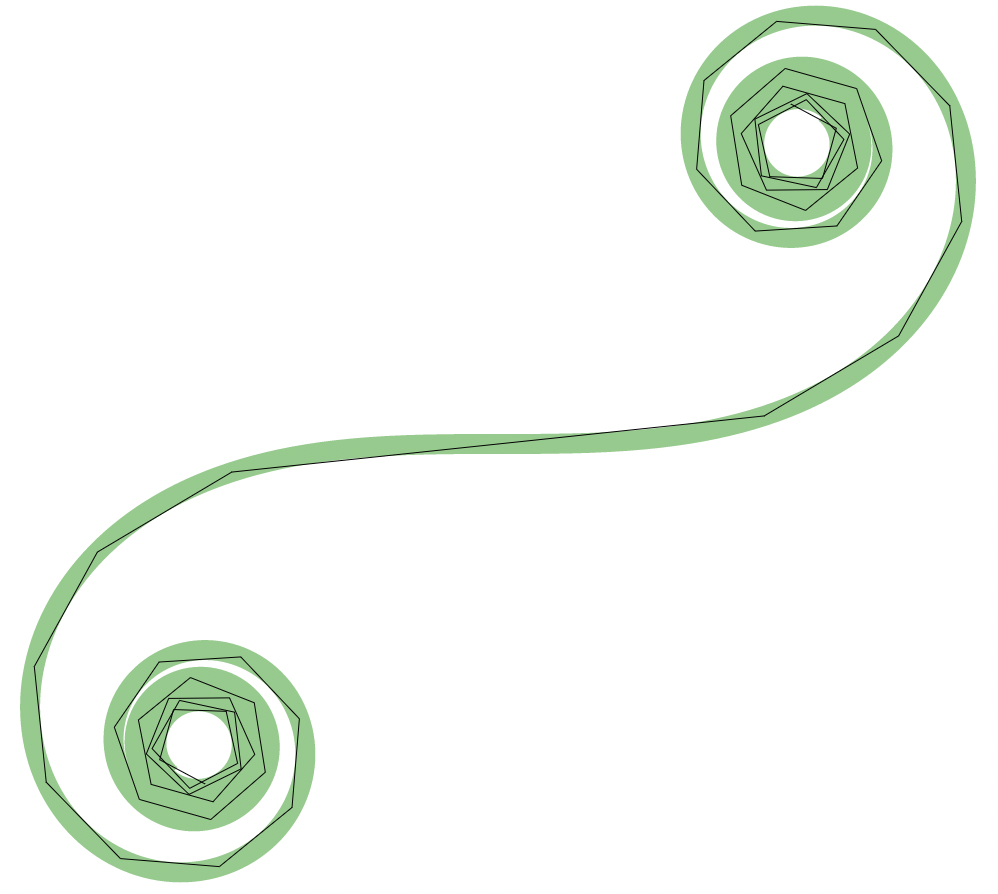
\includegraphics[scale=0.3]{es_flatten}
    \caption{Flattening of an Euler spiral using points spaced by power-law}
    \Description{An Euler spiral along with its flattened representation. The flattened curve has an error}
    \label{fig:es_flatten}
\end{figure}


\section{Euler spirals and their parallel curves}

It is common to approximate cubic Béziers to some intermediate curve format more conducive to offsetting and flattening. A number of published solutions (\cite{Yzerman2020}, \cite{Nehab2020}) use quadratic Béziers, as it is well suited for computation of parallel curves. Even so, this curve has some disadvantages. In particular, it cannot model an inflection point, so the source curve must be subdivided at inflection points.

Like these other approaches, we also use an intermediate curve, but our choice is an Euler spiral. In some ways it is similar to quadratic Béziers -- it also has $O(n^4)$ scaling and is best computed using geometric Hermite interpoliation -- but differs in others. It has no difficulty modeling an inflection point. Further, its parallel curve has a particularly simple mathematical definition and clean behavior regarding cusps.

An Euler spiral segment is defined as having curvature linear in arc length.

The parallel curve of the Euler spiral (also known as ``clothoid'') was characterized by Wieleitner well over a hundred years ago\cite{Wieleitner1907}, and has a straightforward closed-form Cesàro representation, curvature as a function of arc length. TODO: present closed-form solution.

\section{Flattened parallel curves}

The geometry of a stroke outline consists of joins, caps, and the two parallel curves on either side of the input path segemnts, offset by the half linewidth. The former are not particularly difficult to calculate, but parallel curves of cubic Béziers are notoriously tricky. Analytically, is is a tenth order algebraic curve, which is not particularly feasible to compute directly.

Conceptually, generating a flattened stroke outline consists of computing the parallel curve of the input curve segment followed by \emph{flattening,} the generation of a polyline that approximates the parallel curve with sufficient accuracy (which can be measured as Fréchet distance). However, these two stages can be fused for additional performance, obviating the need to store a representation of the intermediate curve.

Using a subpixel Fréchet distance bound guarantees that the rendered image does not deviate visibly from the exact rendering. Another choice would be uniform steps in tangent angle, as chosen by \cite{Kilgard2020}. However, at small curvature, the stroked path can be off by several pixels, and at large curvature there may be considerably more subdivision than needed for faithful rendering.

Proposed image: show circular arcs with polar stroking vs near-optimal flattening.

\subsection{Optimal flattening}

The optimal flattening of a curve, with a maximum error constraint, is as follows. An optimal flattening contains the minimum number of subdivisions required to meet that constraint. Further, the error is the minimum possible with that number of subdivisions.

For a convex curve, the optimal flattening is tractable to compute, though not necessarily very fast. When a curve is monotonic, error is also monotonic with respect to both subdivision points. Thus, any standard root finding technique can find a subdivision with a given error (bisection is the best known, but the ITP method \cite{Oliveira2020} is better). An similar outer loop with a root finding technique can find the error which minimizes the global error for the entire flattening, which, due to monotonicity, is that for which the error of the final segment equals that of the previous segments. Subdividing at the inflection point adds at most one additional point; it is possible to optimize further, but we do not consider that (though the near-optimal flattening we will later present is not subject to this constraint).

\subsection{The subdivision density integral}

The subdivision density for the parallel curve of an Euler spiral, normalized so that its inflection point is at -1 and the cusp of the parallel curve is at 1, is simply $1 - \sqrt{|1-s^2|}$. This function is plotted in Figure\ref{fig:subdiv_density}.

\begin{figure}
    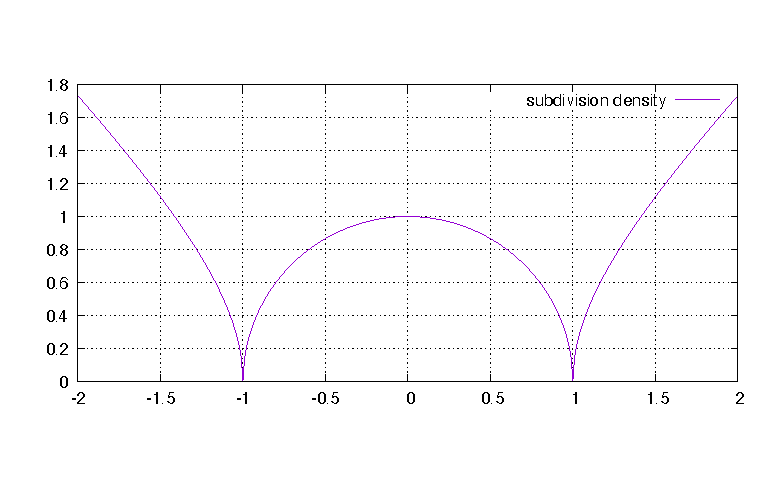
\includegraphics[scale=0.6]{subdiv_density}
    \caption{Subdivision density for the parallel curve of an Euler spiral}
    \Description{A graph of subdivision density. The range from -1 to 1 is a semicircle, and the value from 1 rises sharply from zero to an asymptote of unity slope.}
    \label{fig:subdiv_density}
\end{figure}

The subdivision density integral for the parallel curve of an Euler spiral is given as follows:

\[
    f(x) = \int_0^x\sqrt{|u^2 - 1|} du
\]

This integral has a closed-form analytic solution:

\[
    f(x) = \left\{
        \begin{array}{rl}
            \frac{1}{2}(x\sqrt{|x^2-1|} + \sin^{-1}x) & \text{if } |x| \leq 1 \\
            \frac{1}{2}(x\sqrt{|x^2-1|} - \cosh^{-1}x + \frac{\pi}{4}) & \text{if } x \geq 1
        \end{array}
    \right.
\]

Values for $x<-1$ follow from the odd symmetry of the function. 


\subsection{Approximation of the subdivision density integral}

The subdivision density integral [TODO: probably should use section or equation number reference] is fairly straightforward to compute in the forward direction, but not invertible using a straightforward closed-form equation. Numerical techniques are possible, but require multiple iterations to achieve sufficient accuracy, so are slower. In this subsection, we present a straightforward and accurate approximation, based on piecewise easily invertible functions. If higher flattening quality is desired at the expense of slower computation, this approximation can be used to determine a good initial value for numeric techniques; two iterations of Newton solving are enough to refine this guess to within 32-bit floating point accuracy.

The approximation is given as follows:

\[ 
    f_\mathit{approx}(x) = \left\{
        \begin{array}{rl}
            \frac{\sin c_1 x}{c_1} & \text{if } x < 0.8 \\
            \frac{\sqrt{8}}{3}(x-1)^{1.5} + \frac{\pi}{4} & \text{if } 0.8 \leq x < 1.25 \\
            0.6406x^2 - 0.81x + c_2 & \text{if } 1.25 \leq x < 2.1 \\
            0.5x^2 - 0.156x + c_3 & \text{if } x \geq 2.1
        \end{array}
        \right.
\]
\[
    \begin{array}{ll}
        c_1 = & 1.0976991822760038 \\
        c_2 = & 0.9148117935952064 \\
        c_3 = & 0.16145779359520596
    \end{array}
\]

The primary rationale for the constants is for the approximation to be continuous. The other parameters were determined empirically; further automated optimization is possible but is unlikely to result in dramatic improvement. Further, this approximation is given for positive values. Negative values follow by symmetry, as the function is odd.

The exact integral and the approximation given above are shown in Figure~\ref{fig:espc}. Visually, it is clear that the agreement is close, and in numerical testing the worst case discrepancy between approximate and exact results is approximately 6\%.

\begin{figure}
    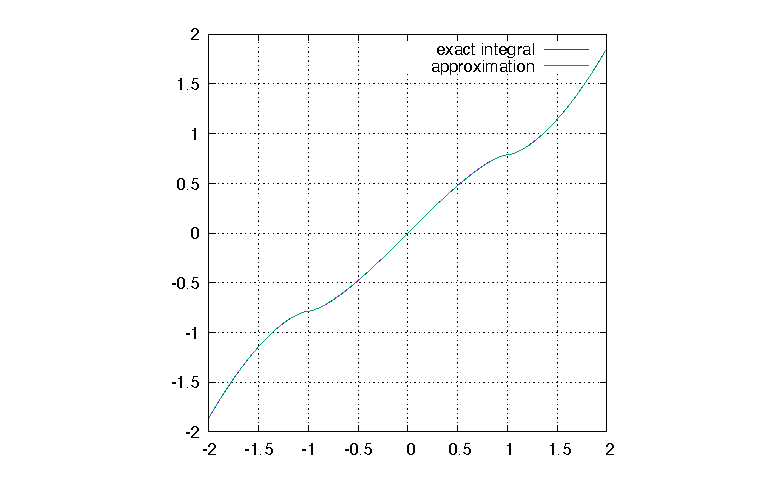
\includegraphics{espc}
    \caption{Integral of subdivision density for Euler spiral parallel curve, and its approximation}
    \Description{A graph of the integral of subdivision density. It is a wriggly diagonal line, with flat parts at -1 and 1. The approximation is nearly indistinguishable from the exact value.}
    \label{fig:espc}
\end{figure}

\section{Error metrics for approximation by arcs}

The problem of approximating a curve by a sequence of arc segments has extensive literature, but none of the published solutions are quite suitable for our application. The specific problem of approximating an Euler spiral by arcs is considered in \cite{Meek2004} using a ``cut then measure'' adaptive subdivision scheme, but their solution has poor quality; it scales as $O(1/n^2)$, while $O(1/n^3)$ is attainable. The result was improved ``slightly'' by \cite{Narayan2014}. The literature also contains optimal results, namely \cite{Maier2014} and \cite{Nuntawisuttiwong2021}, but at considerable cost; both approaches claim $O(n^2)$ time complexity. The through-line for all these results is that they are solving a harder problem, adopting the constraint that the generated arc sequence is $G^1$ continuous. While desirable for many applications, for simply rendering a stroked outline, it is not needed. Even with this constraint relaxed, the angle discontinuities of an arc approximation are tiny compared to the flattening to lines.

% I also expect that the Fréchet distance error of a solution not constrained by G1 continuity will be better by some constant factor (somewhere around 2-4, just as a gut feeling) than the G1-continuous optimum solution. This is a major reason why we have such favorable segment counts, even in comparison to Euler spirals. However, providing evidence for that claim feels more in scope for another paper.

Our approach is based on a simple error metric, similar in flavor to the one for flattening to line segments. The details of the metric (in particular, tuning of constants) were obtained empirically, though we suspect that more rigorous analytic bounds could be obtained. In practice it works very well indeed; the best way to observe that is an interactive testing tool, which is provided in the supplemental materials.

The proposed error metric is as follows. The estimated distance error for a curve of length $\hat{s}$ is:

\[
    d \approx \frac{1}{120}\left(\int_0^{\hat{s}} \sqrt[3]{|\kappa'(s)|}ds \right)^3
\]

For an Euler spiral segment, $\kappa'(s)$ is constant and thus this error metric becomes nearly trivial. With n subdivisions, the estimated distance is simply $\frac{s^3\kappa'}{120n^3}$. Solving for $n$, we get $n = s\sqrt[3]{\frac{|\kappa'|}{120d}}$ subdivisions, and those are divided evenly by arc length, as the subdivision density is constant across the curve, just as is the case for flattening arcs to lines.

TODO: image. This will likely strongly resemble Fig. 8a from Narayan2014.

Remarkably, the approximation of an Euler spiral parallel curve by arc segments is almost as simple as that for Euler spirals to arcs. As in flattening to lines, the parameter for the curve is the arc length of the originating Euler spiral. The subdivision density is then constant, and only a small tweak is needed to the formula for computing the number of subdivisions, taking into account the additional curvature variation from the offset by $h$ (the half line-width). The revised formula is:

\[
    n = s\sqrt[3]{\frac{|\kappa'|(1+0.4|hs\kappa'|)}{120d}}
\]

This formula was determined empirically by curve-fitting measured error values from fitting Euler spiral parallel curves to arcs, but was also inspired by applying the general error metric formula to the analytical equations for Euler spiral parallel curve, and dropping higher order terms. A more rigorous derivation, ideally with firm error bounds, remains as future work.

One consequence of this formula is that, since $h$ appears under absolute value, the same arc approximation can be used for both sides of a stroke.

% Make improved quality claim here? I think it may be too subtle.

\section{Evolutes}

In the principled, correct specification for stroking\cite{Nehab2020}, parallel curves are sufficient only for segments in which the curvature does not exceed the reciprocal half width. When it does, additional segments must be drawn, including evolutes of the original curve. In general, the evolute of a cubic Bézier is a very complex curve, requiring approximation techniques. By contrast, the evolute of an Euler spiral ($\kappa = as$) is another spiral with a simple Cesàro equation, namely $\kappa = -a^{-1}s^{-3}$, an instance of the general result that the evolute of a log-aesthetic curve is another log-aesthetic curve\cite{Yoshida2012}.

Flattening this evolute is also straightforward; the subdivision density is proportional to $s^{-0.5}$ where $s$ is the arc length parameter of the underlying Euler spiral (and translated so $s = 0$ is the inflection point). Thus, the integral is $2\sqrt{s}$, and the inverse integral is just squaring. Thus, flattening the evolute of an Euler spiral is simpler than flattening its parallel curve.

TODO: figure showing ES, its evolute, and subdivision points for flattening.

\section{Conversion from cubic Béziers to Euler spirals}

The Euler spiral segment representation of a curve is useful for computing near-optimal flattened parallel curves, but standard APIs and document formats overwhelmingly prefer cubic Béziers as the path representation.

Many techniques for stroke expansion described in the literature apply some lowering of cubic Bézier curves to a simpler curve type, more tractable for evaluating parallel curve. Computing parallel curves directly on cubic Bézier curve segments is not very tractable. In particular, the widely cited Tiller-Hanson algorithm\cite{Tiller1984} performs well for quadratic Béziers but significantly worse for cubics.

% TODO: the discussion of adaptive subdivision maybe duplicates the earlier section on "measure then cut."

A typical pattern for converting from one curve type to another is \emph{adaptive subdivision.} (TODO: is there a good general reference for this?) An approximate curve is found in the parameter space of the target curve family. The error of the approximation is measured. If the error exceeds the specified tolerance, the curve is subdivided (typically at $t = 0.5$), otherwise the approximation is accepted. Subdivisions are also indicated at special points; for example, since quadratic Béziers cannot represent inflection points, and geometric Hermite interpolation is numerically unstable if the input curve is not convex, lowering to quadratic Béziers also requires calculation of inflection points and subdividing there. A good example of this pattern is Nehab\cite{Nehab2020}. One advantage of Euler spirals over quadratic Béziers is that they can represent inflection points just fine, so it is not necessary to compute those for additional subdivision.

The approach in this paper is another variant of adaptive subdivision, with two twists. First, it's not necessary to actually generate the approximate curve to measure the error. Rather, a straightforward closed-form formula accurately predicts it. The second twist is that, since compute shader languages on GPUs typically don't support recursion, the stack is represented explicitly and the conceptual recursion is represented as iterative control flow. This is an entirely standard technique, but with a clever encoding the entire state of the stack can be represented in two words, each level of the stack requiring a mere single bit.

\subsection{Error prediction}

A key step in approximating one curve with another is evaluating the error of the approximation. A common approach (used in \cite{Nehab2020} among others) is to generate the approximate curve, the measure the distance, often by sampling at multiple points on the curve. All this is potentially slow, with the additional risk of underestimating the error due to undersampling.

Our approach is different. In short, we perform a straightforward analytical computation to accurately estimate the error. Our approach to the error metric has two major facets. First, we obtain a cubic Bézier which is a very good fit to the Euler spiral, then we estimate the distance between that and the source cubic. Due to the triangle inequality, the sum of these is a conservative estimate of the true Fréchet distance between the cubic and the Euler spiral.

For mathematical convenience, the error estimation is done with the chord normalized to unit distance; the actual error is scaled linearly by the actual chord length.

The cubic Bézier approximating the Euler spiral is that with the distance of each control point from the endpoint is $d = \frac{2}{3(1 + \cos \theta)}$, where $\theta$ is the angle of the endpoint tangent relative to the chord. This is a generalization of the standard approximation of an arc. It should be noted that this is not in general the closest possible fit, but it is computationally tractable and has near-uniform parametrization. In general it has quintic scaling; if an Euler spiral segment is divided in half, the error of this cubic fit decreases by a factor of 32. A good estimate of this error is:

\[
    4.6255\times10^{-6}|\theta_0+\theta_1|^5 + 7.5\times10^{-3}|\theta_0+\theta_1|^2|\theta_0-\theta_1|
\]

Possible image for this: the heatmap from the cleaner parallel curves blog post.

The distance between two cubic Bézier segments can be further broken down into two terms; in most cases, the difference in area accurately predicts the Fréchet distance between the curves. Two cubic Béziers with the same area and same tangents tend to be relatively close to each other, but there is some error stemming from the difference in parametrization. Area of a cubic Bézier segment is straightforward to compute using Green's theorem:

\[
    a = \tfrac{3}{20}(2d_0\sin \theta_0 + 2d_1\sin \theta_1 - d_0 d_1\sin(\theta_0+\theta_1))
\]

The conservative Fréchet distance estimate is 1.55 the absolute difference in area between the source cubic and the Euler spiral approximation. The final term for imbalance is as follows, with $\bar{d}_0$ and $\bar{d}_1$ representing the distance from the endpoints of the Euler approximation and $d_0$ and $d_1$ the corresponding distance in the source cubic segment, as in the area calculation above:

\[
    (0.005|\theta_0+\theta_1| + 0.07|\theta_0 - \theta_1|)\sqrt{(\bar{d}_0 - d_0)^2 + (\bar{d}_1 - d_1)^2}
\]

The total estimated error is the sum of these three terms. We have validated this error metric in randomized testing. For values of $\theta$ between $0$ and $0.5$, and values of $d$ between $0$ and $0.6$, this estimate is always conservative, and it is also tight: over Bézier curves generated randomly with parameters drawn from a uniform distribution this range, the mean ratio of estimated to true error is 1.656.

% Note about supplemental materials. This ratio is produced by examples/euler3 in Raph's local branch of euler_err_experiment of kurbo (git 99b00). This should be cleaned up and moved into the code repo.

\subsection{Geometric Hermite interpolation}

Given tangent angles relative to the chord, finding the Euler spiral segment that minimizes total curvature variation is a form of geometric Hermite interpolation. There are a number of published solutions to this problem, all involving nontrivial numerical solving techniques: gradient descent\cite{Kimia2003}, bisection\cite{Walton2009}, or Newton iteration\cite{Connor2014}. Our approach is much more direct. We observe that the Euler spiral parameters are a smooth function of the two input parameters, and determine a 2D Taylor's series for this function. Many of the terms are zero because of symmetry. Preserving terms up to 7th order provides excellent accuracy (TODO: quantify more carefully) with modest computational expense.

TODO: A good cite for this is \cite{Reif2021}. Our solution is similar in flavor, but is more precise at modest cost as it contains more polynomial terms.

TODO: the technique used is a refinement of what was sketched in the Python notebook attached to the "cleaner parallel curves with Euler spirals" blog post. It's basically a 2D Taylor's series. Previously we had the secant method from section 8.2 of my thesis; not sure whether we want to cite that in the submission for anonymity reasons. It's functionally pretty similar to the \cite{Connor2014} reference.

\subsection{Unrolled recursion}

The entire recursion stack for adaptive subdivision can be represented in two words: dt and scaled\_t0. The range is dt * scaled\_t0 .. dt * (scaled\_t0 + 1). Initial values of 1 and 0 represent the range (0, 1). Pushing the stack, subdividing the range in half, is representing by halving dt and doubling scaled\_t0, which leaves the start of the range invariant but its size halved. After accepting an approximation, the next range is determined by incrementing scaled\_t0, then repeatedly popping the stack by doubling dt and halving scaled\_t0, as long as the latter is odd. This can in fact be achieved without iteration by using the ``count trailing zeros'' intrinsic.

\section{Future work}

\begin{itemize}
    \item The GPU implementation sequentializes some work that could be parallel, and is thus not as well load-balanced as it might be. An appealing future direction is to split the pipeline into separate stages, executed by the GPU as nodes in a work graph\cite{Patel2024}. This structure is appealing because load balancing is done by hardware.

    \item Many of the error metrics were empirically determined. The mathematical theory behind them should be developed more rigorously, and that process will likely uncover opportunities to fine-tune the technique.
\end{itemize}

\section{Discussion}

\bibliographystyle{ACM-Reference-Format}
\bibliography{paper}

\end{document}
